\chapter{Creating an Efficient Database Infrastructure for Discovery of Real Materials Exemplified with High Entropy Alloys} \label{chap:ultera}

\section{Introduction} \label{ultera:sec:intro}

Compared to atomic structures, which are precisely defined, data on "real" materials which were physically made in a lab tends to be (a) much less homogeneous in terms of \textit{how} it is reported and (b) much less defined in terms of the \textit{completeness} of description, i.e., many critical parameters like phases present can be missing or misreported due to a plethora of reasons including lack of equipment, limited precision, or human errors. Because of these, handling 

\cite{Debnath2021GenerativeAlloys}
\cite{Debnath2023ComparingAlloys}
\cite{Li2024DesignExperiments}

\begin{figure}[H]
    \centering
    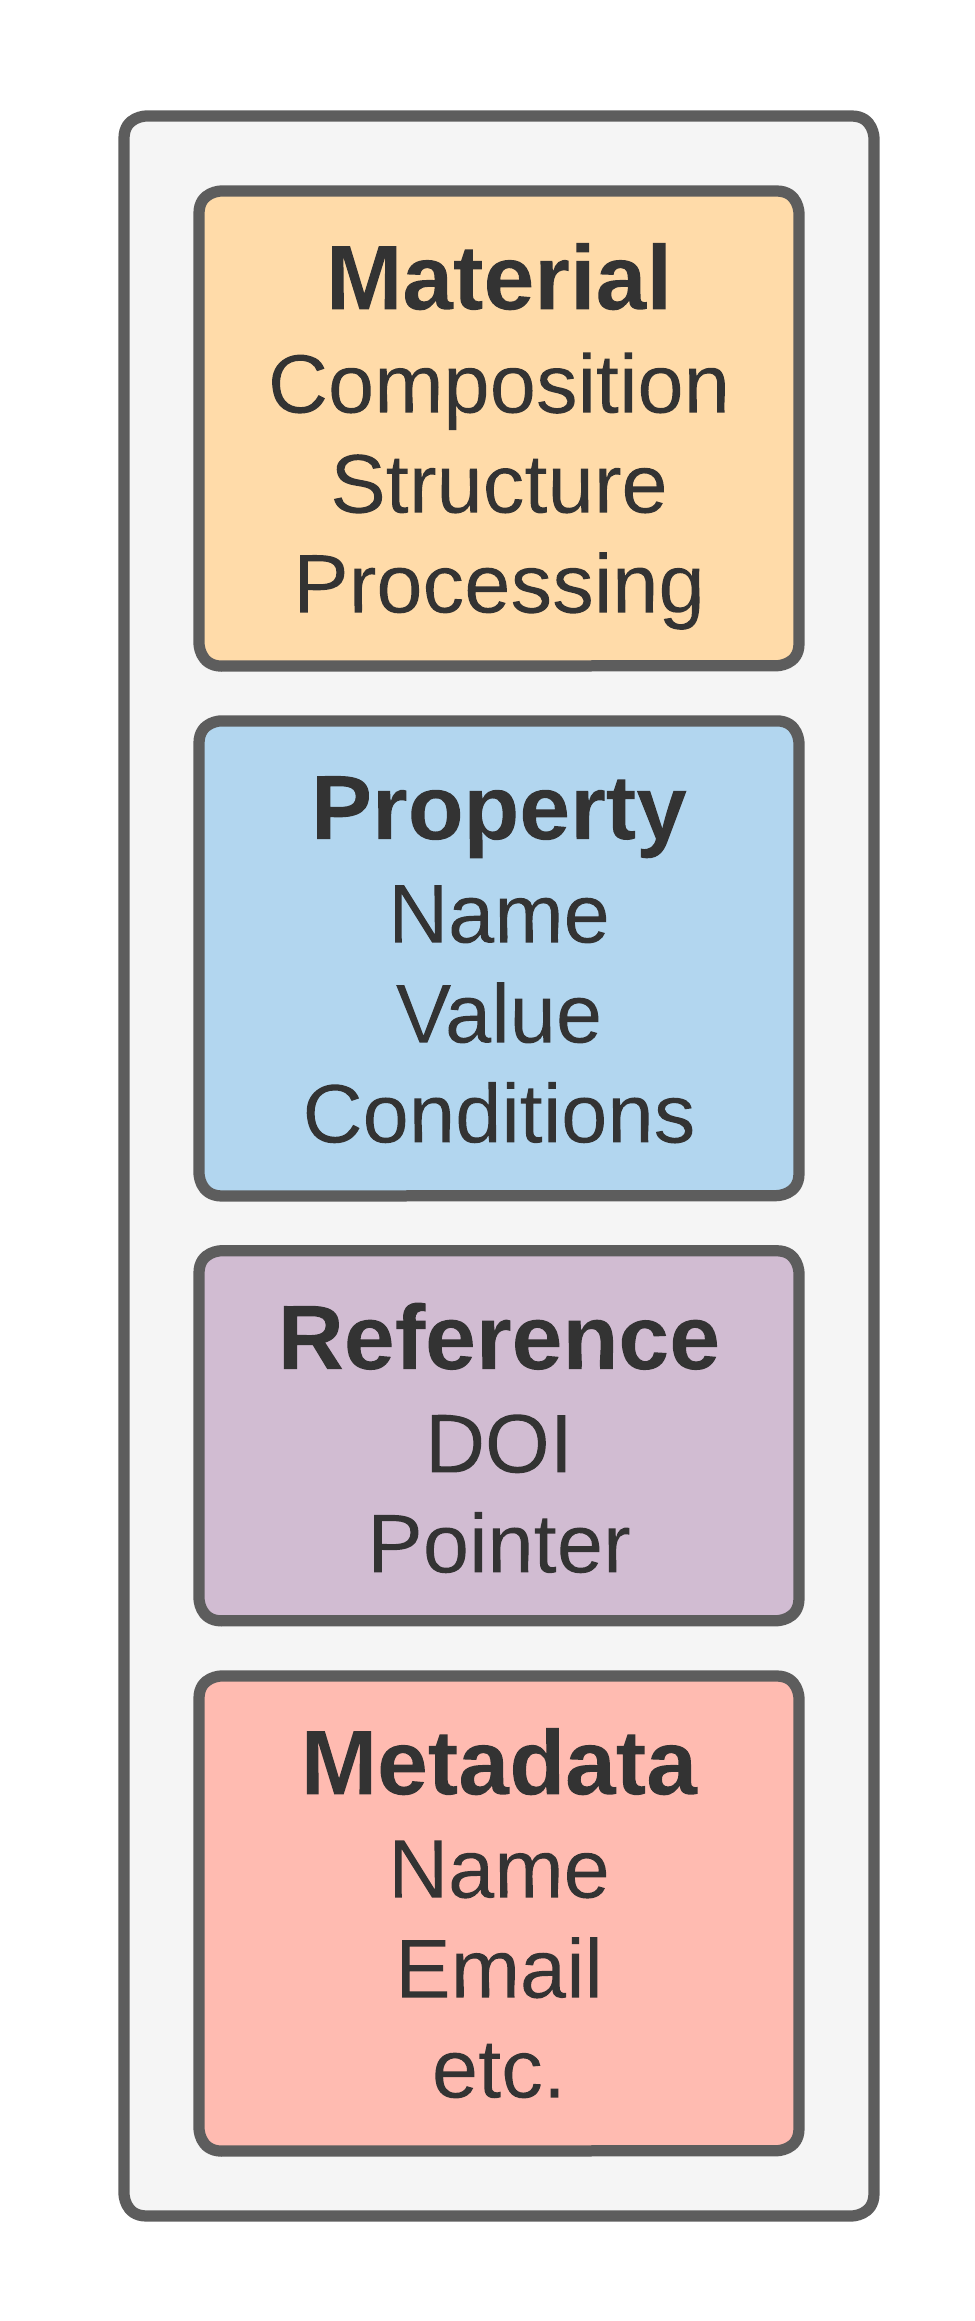
\includegraphics[width=0.2\textwidth]{ultera/ULTERA Data Detail_material.png}
    \caption{Underlying core data overview.}
    \label{ultera:fig:material}
\end{figure}


\section{Dataset} \label{ultera:sec:datadescription}
\newcommand{\statisticstime}{April 2024}

The dataset of the ULTERA Database has been manually collected through efforts of several ULTERA team members specializing in different properties, augmented with a few manually collected literature datasets processed through curation and aggregation data pipelines described in Section \ref{ultera:sec:pipeline}. All data was then further curated through \texttt{PyQAlloy} software described in Chapter \ref{chap:pyqalloy}, typically resulting in $5-10\%$ of the data points being modified to match original publications or removed.

After all the data processing steps, which generally reduced the number of datapoints and prioritized original studies over larger collections, as of \statisticstime, $\approx54\%$ of the property datapoints has been collected internally by ULTERA team, $\approx39\%$ from internally-improved version of dataset by \citet{Borg2020ExpandedAlloys}, $\approx5\%$ from \citet{Yang2022AHardness}, and $\approx3\%$ from \citet{Wang2023SearchingExperiments}. Collectively, over 550 scientific publications have been parsed to arrive at nearly 7,000 individual \textit{experimental} property datapoints, with further 500 coming from computer-based methods, belonging to nearly 3,000 unique materials spanning nearly 2,000 distinct chemical compositions, as presented in Figure~\ref{ultera:fig:dashboard}, which can be accessed in its most current form under \href{https://ultera.org}{ultera.org} project website.

\begin{figure}[H]
    \centering
    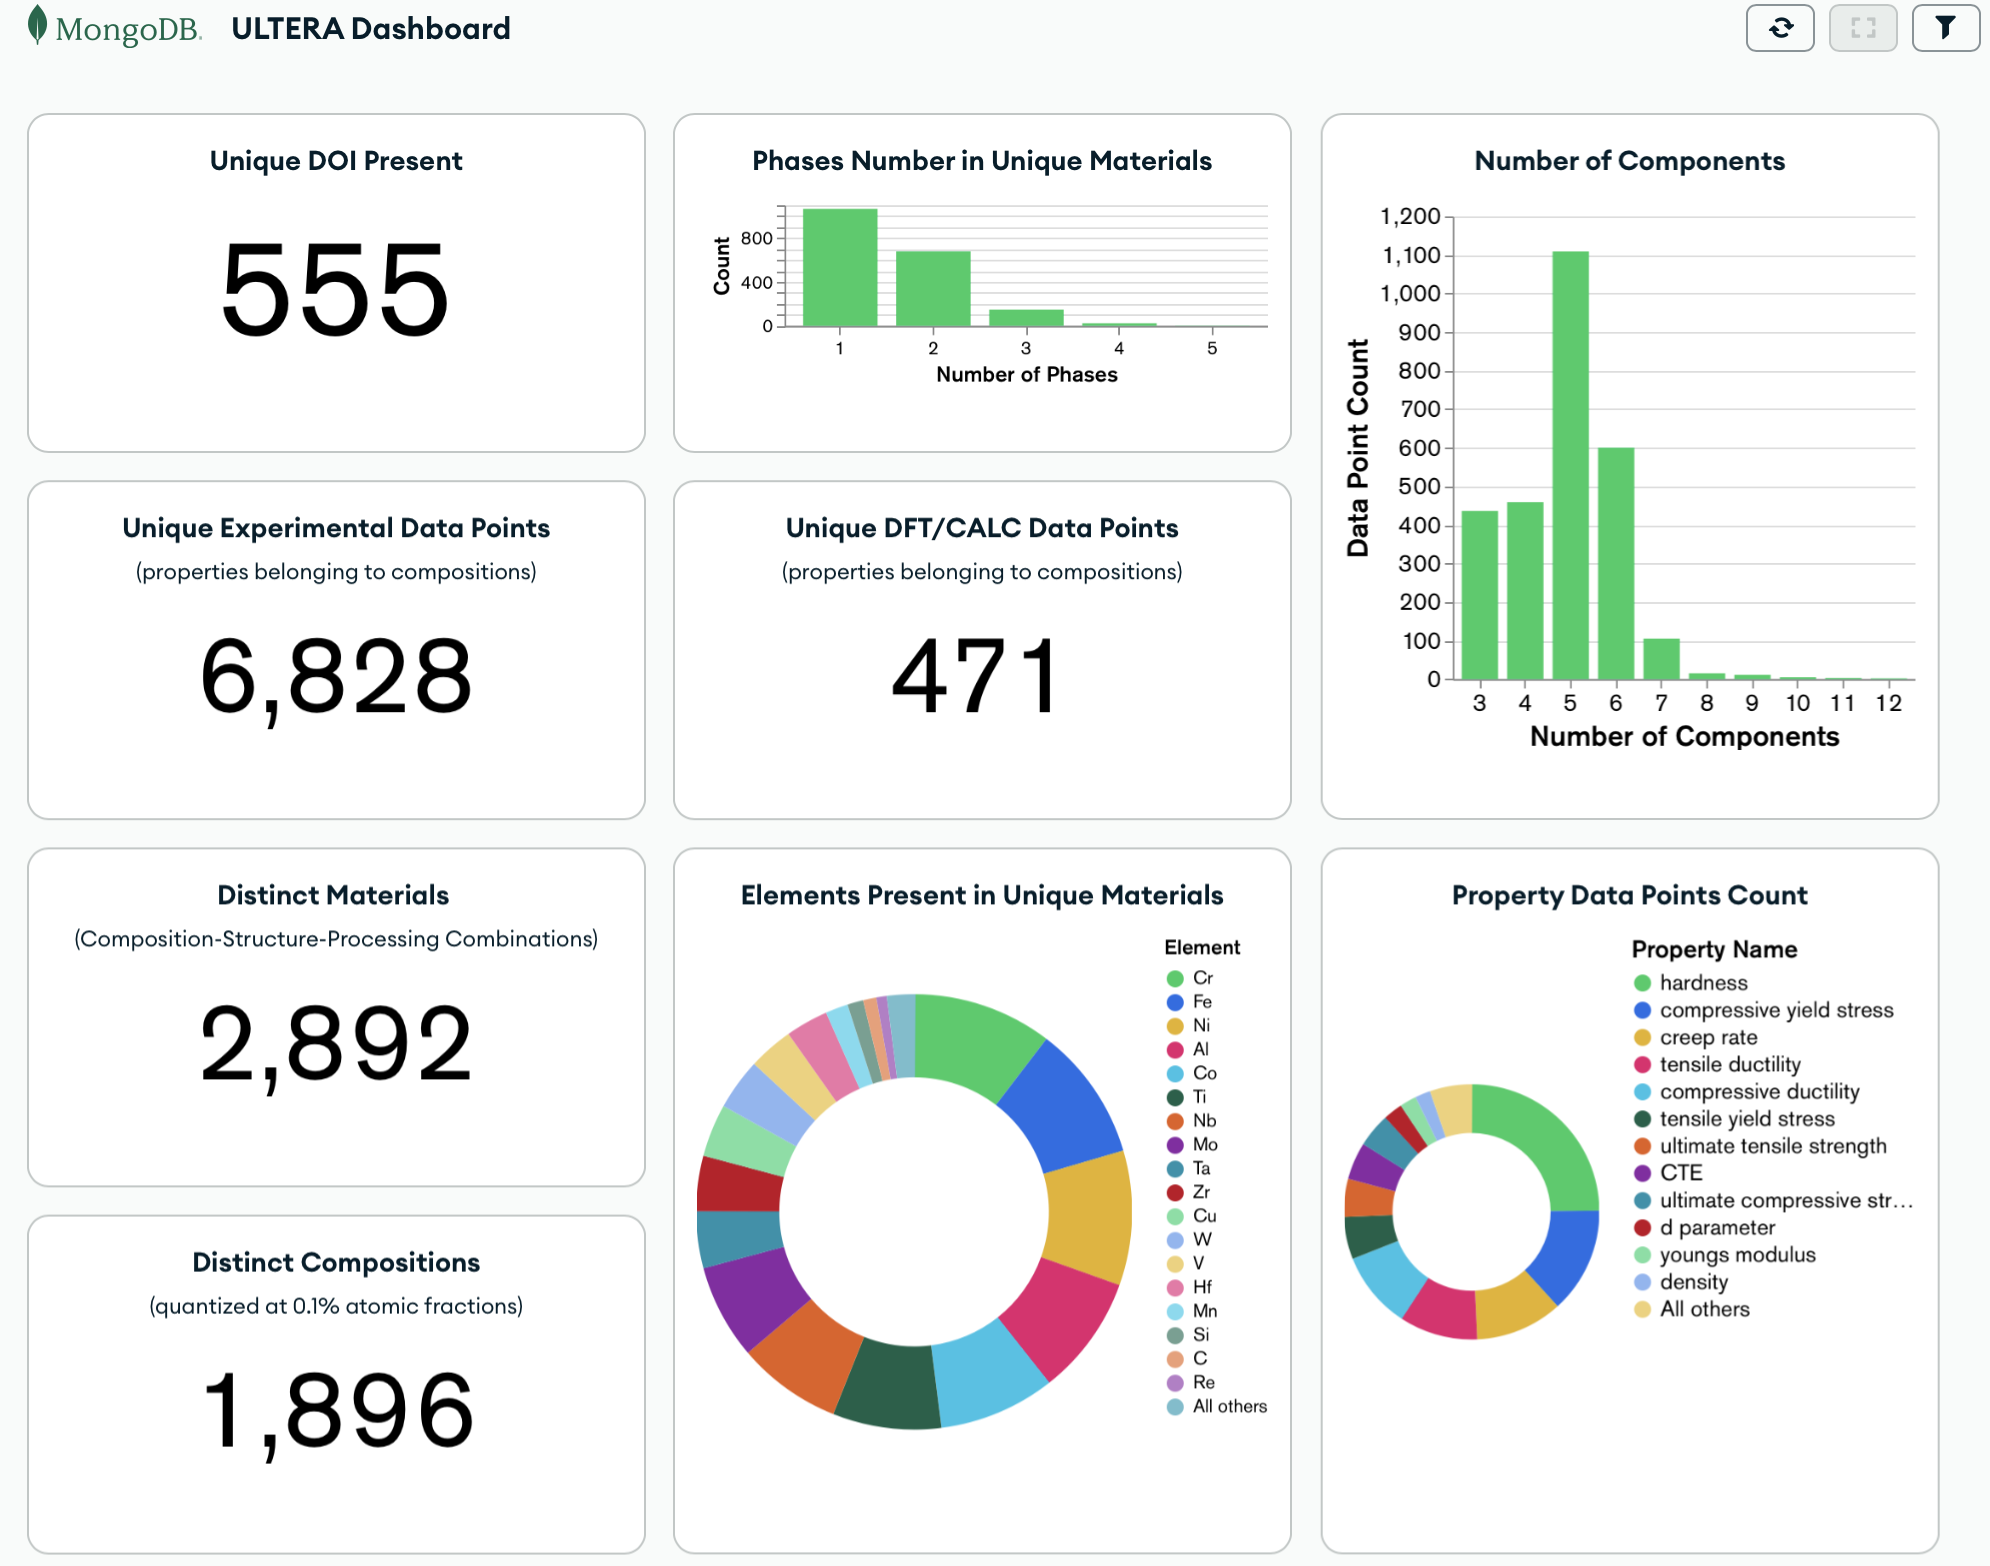
\includegraphics[width=0.95\textwidth]{ultera/ULTERA_Dashboard.png}
    \caption{The main section of \texttt{ULTERA} Database dashboard at \href{https://ultera.org}{ultera.org}; presents statistics as of \statisticstime. All included figures are live and automatically recalculated every 1h. They are interactive allowing users to, e.g., select, highlight, or export the plot data in machine-readable format.}
    \label{ultera:fig:dashboard}
\end{figure}

As depicted in the bottom part of Figure~\ref{ultera:fig:dashboard}, the dataset covers a diverse set of (a) properties and (b) chemical elements. The property set spans 12 with at least 130 datapoints present, with 10 coming from experiments and 2 from computation, with the most common being hardness ($24.6\%$), tensile or compressive ductility ($19.7\%$), tensile or compressive yield stress ($18.9\%$), creep rate ($11.3\%$), and compressive or tensile ultimate strength ($9.1\%$).

The chemical space coverage spans 37 elements, with no bias towards a small subset of them, that most commonly co-occur in 5-component systems, as shown in Figure~\ref{ultera:fig:dashboard}. Out of the chemical elements, 20 are present in at least 80 unique alloys, as listed in Figure~\ref{ultera:fig:chemistries}, making them suitable for ML studies.

\begin{figure}[H]
    \centering
    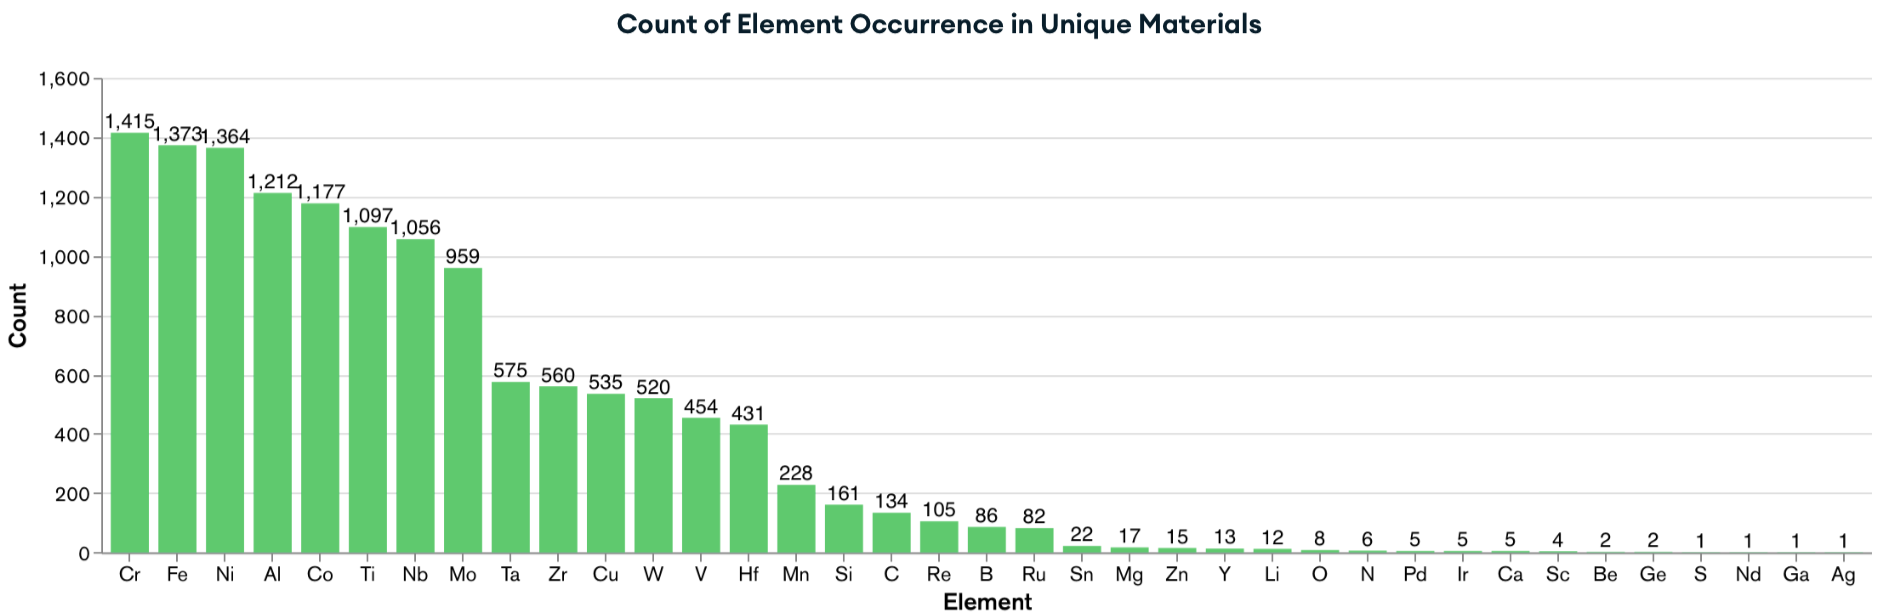
\includegraphics[width=0.95\textwidth]{ultera/ultera_Chemistries.png}
    \caption{Chemical elements in the unique materials collection of the ULTERA Database as of \statisticstime. Please note that the same formula-processing-structure triplet can often be reported by many groups and is counted here as 1 point.}
    \label{ultera:fig:chemistries}
\end{figure}

For each experimental datapoint, the Crossref (\href{https://www.crossref.org}{crossref.org}) service is automatically queried based on the associated DOI (once per unique DOI) to retrieve a set of metadata associated with the study. This allows ULTERA to also be analyzed in terms of time-distribution of the experimental data which can reveal trends in the community regarding its research output, as shown in Figure~\ref{ultera:fig:publicationyears}, or to analyze trends in the explored alloys chemical spaces over the years. The significance of the latter will likely grow in the future, as it can prevent implicit biases into exploration of what "should work", which can limit innovation and design space exploration.

\begin{figure}[H]
    \centering
    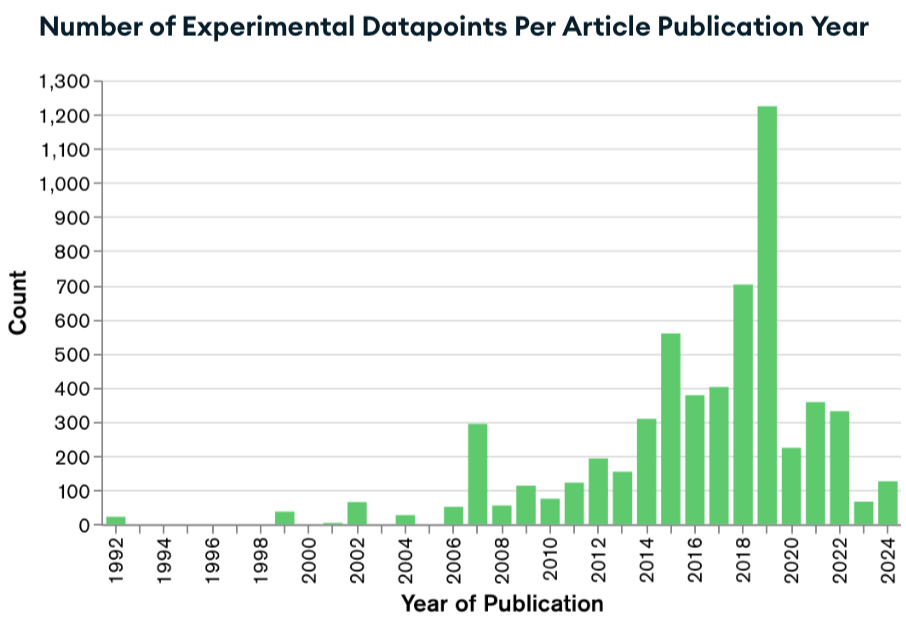
\includegraphics[width=0.6\textwidth]{ultera/ultera_PublicationYear.png}
    \caption{Number of experimental datapoints collected in ULTERA as of \statisticstime vs the year they were published, showing rapid growth. The lower numbers in the last 5 years reported can be attributed to significant portion of the data coming from compilations delayed by 1-3 years and height of COVID pandemic in 2020 delaying experiments.}
    \label{ultera:fig:publicationyears}
\end{figure}

Lastly, it is critically beneficial that every datapoint inserted into the ULTERA's data ecosystem is automatically extended through a number of data homogenization tools, machine learning models, and empirical models, described in later sections, which become immediately available to both modeling researchers (through an API) and data end-users. While much less accurate compared to proper investigations, their complete (or near-complete) coverage is a unique asset, as it puts all materials in the same context, visualizing trends over the entire database, as shown in Figure~\ref{ultera:fig:insights}.

\begin{figure}[H]
    \centering
    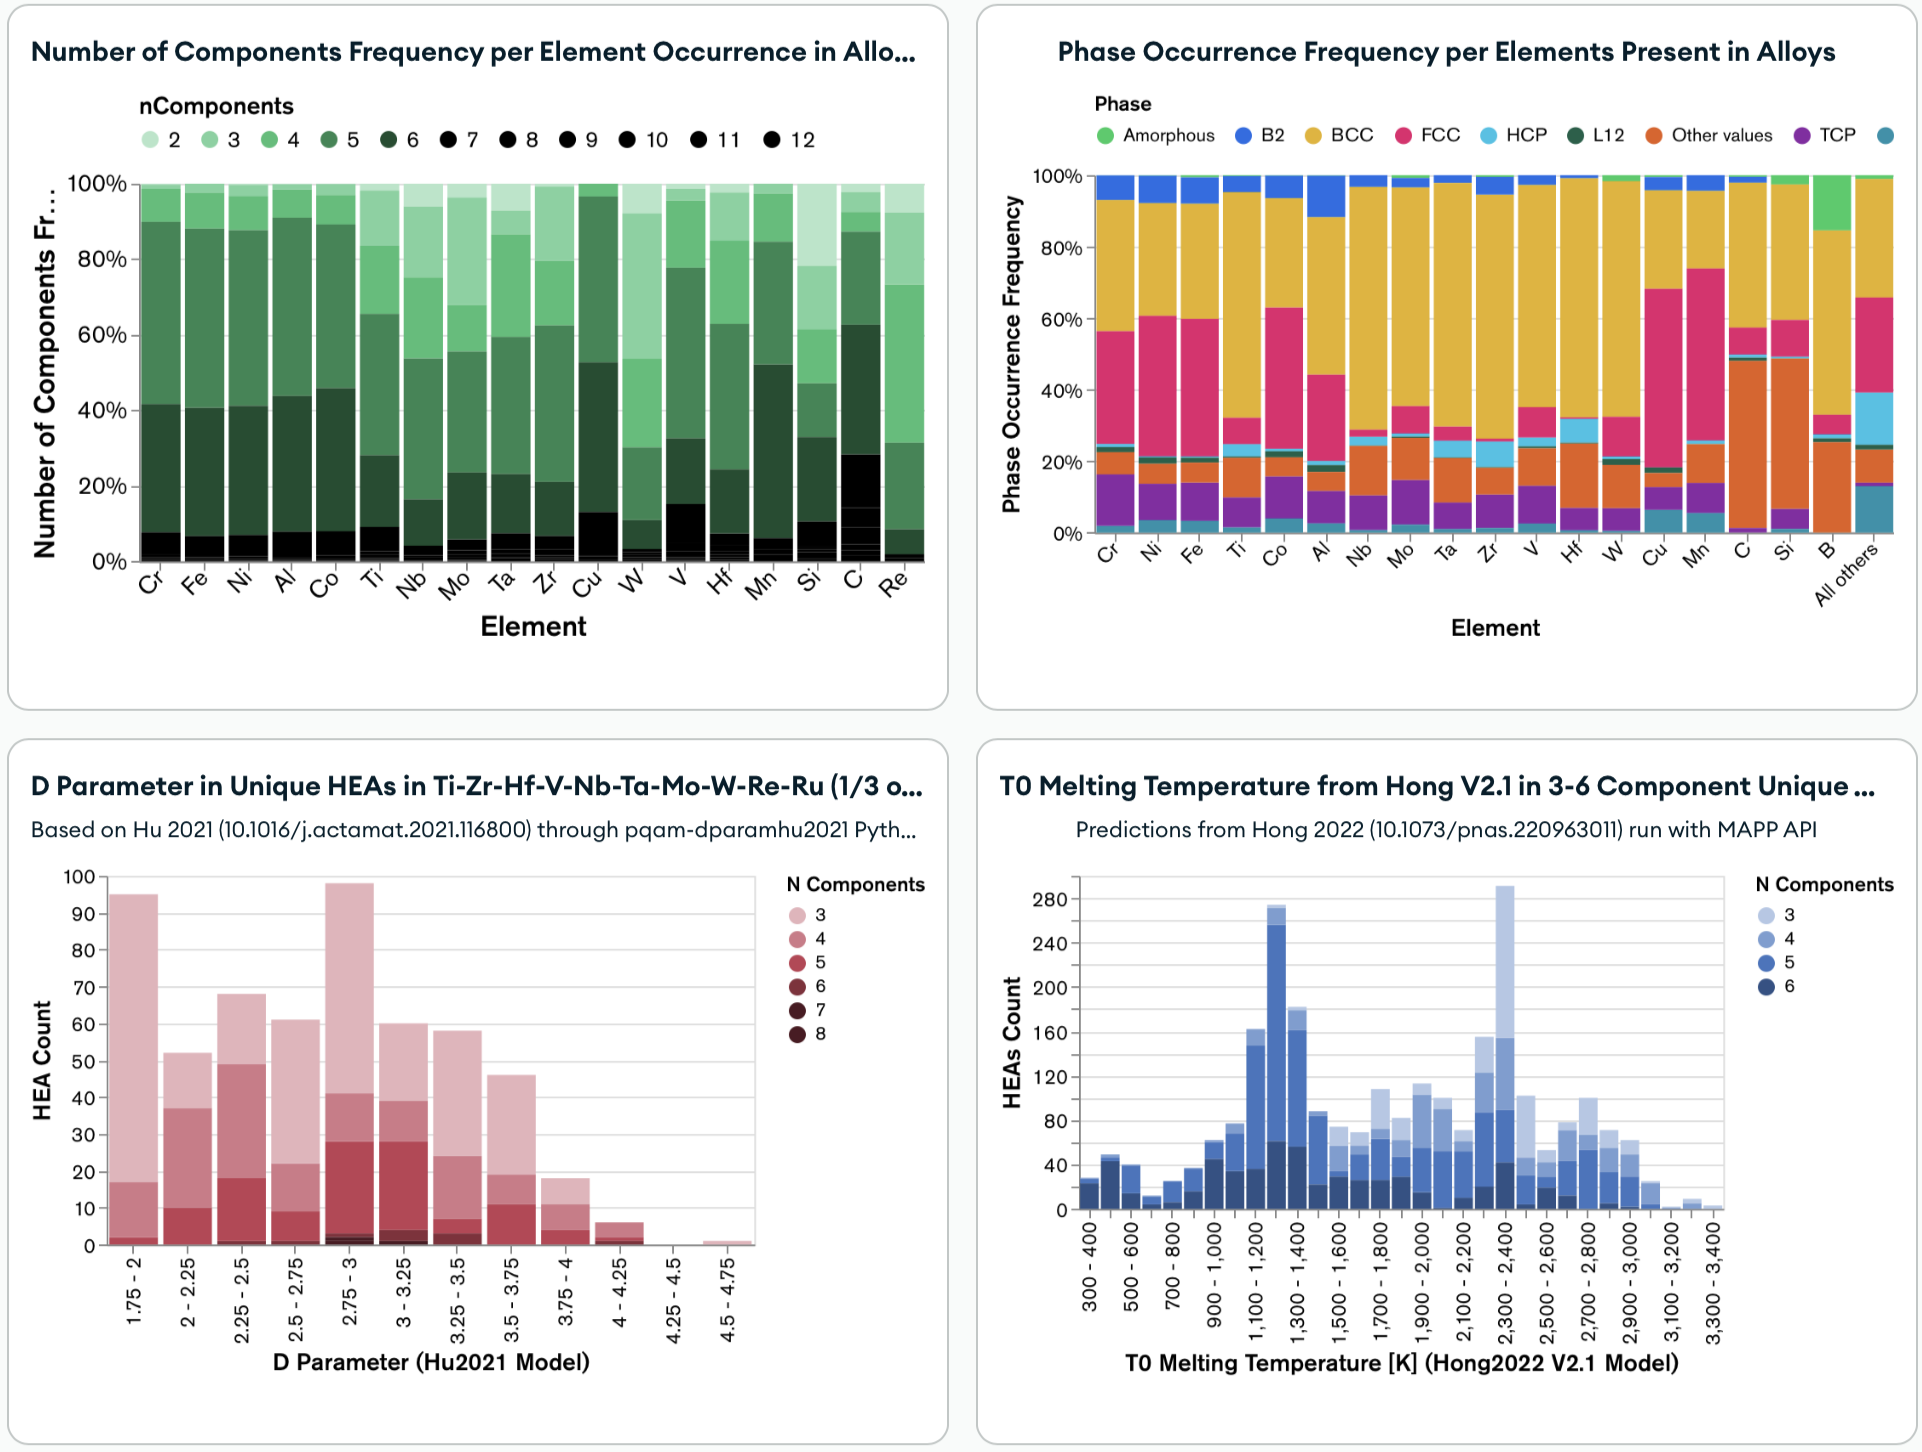
\includegraphics[width=0.95\textwidth]{ultera/ULTERA_Insights.png}
    \caption{A large compiled dataset allows insights into prior expert knowledge driving the discovery and possible biases models generating new alloys will be subject to. The automated data infrastructure, described in Section \ref{ultera:sec:infrastructure}, enables efficient deployment of many tools, such as community models described in Subsection \ref{ultera:ssec:communitymodels}.}
    \label{ultera:fig:insights}
\end{figure}


\section{Alloy Discovery Infrastructure} \label{ultera:sec:infrastructure}

The ULTERA Alloy Discovery Infrastructure, first published conceptually in 2021 \cite{Debnath2021GenerativeAlloys}, is based on a multi-loop paradigm, where \emph{literature} loop, which collects and extracts as much past knowledge as possible, feeds into the \emph{inverse design} loop, which proposes new alloys based on machine learning (ML) and articifical intelligence (AI) techniques, which are lastly verified experimentally and computationally through \emph{validation loop}, while forward models in the \emph{predictive loop} are developed to fill in the gaps in the knowledge, as depicted in Figure~\ref{ultera:fig:dataloops}. All of the loops are handled by largely independent sub-teams with specific expertise, while the communication of the data between them is facilitated through the ULTERA Database, from which novel alloys are "harvested" after verification.

\begin{figure}[H]
    \centering
    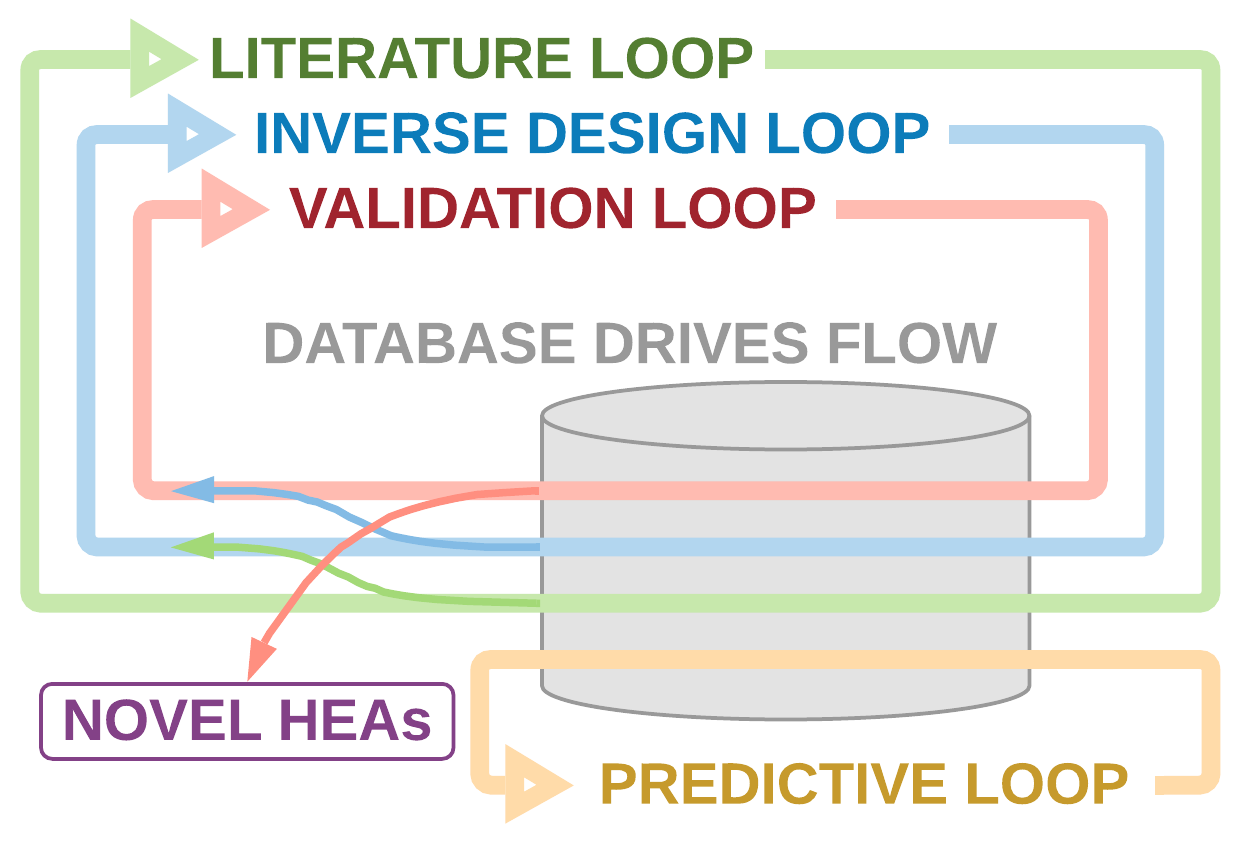
\includegraphics[width=0.5\textwidth]{ultera/PersepctivePaper_DataFlow_V2.png}
    \caption{Four \emph{data loops} associated with different parts of the alloy discovery efforts and the database driving information flow between them to arrive at novel high entropy alloys.}
    \label{ultera:fig:dataloops}
\end{figure}

\begin{figure}[H]
    \centering
    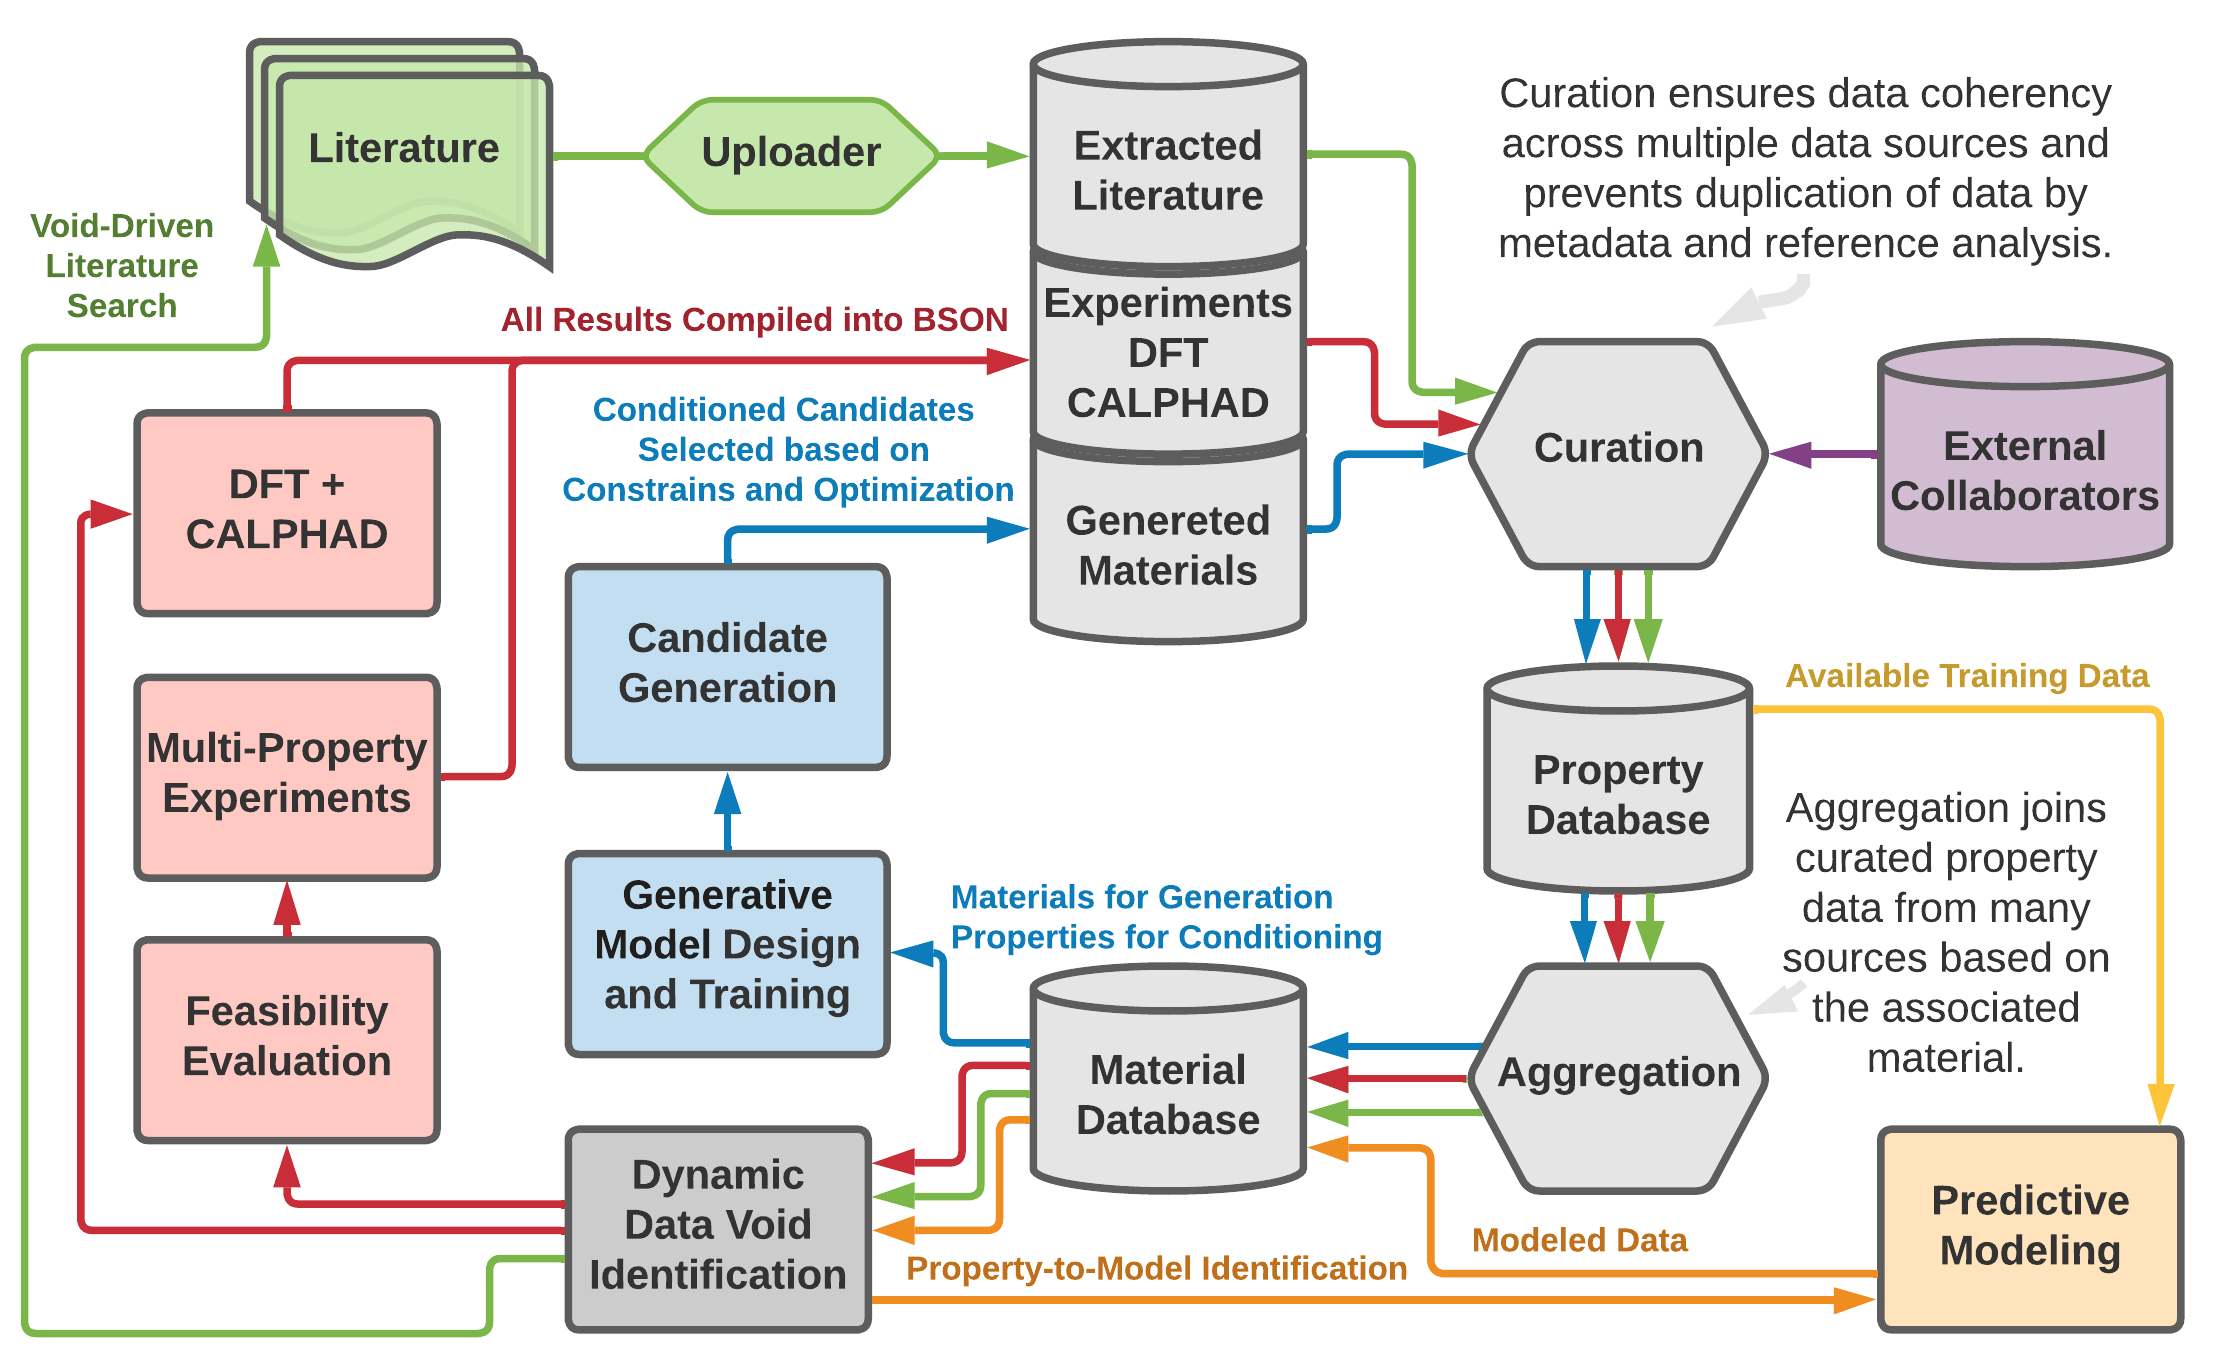
\includegraphics[width=0.9\textwidth]{ultera/PersepctivePaper_Ecosystem_V6.png}
    \caption{Big picture schematic of the ULTERA Data Infrastructure composed of the literature loop (green) collecting available external knowledge from many sources, the predictive loop (orange) filling in the gaps in current state of knowledge with modeling data, the generative loop (blue) proposing new candidate alloys to evaluate, validation loop (red) performing calculations and experiments to validate candidates. In the process databases are created, containing \texttt{CURATED} subset of materials property data, then \texttt{AGGREGATED} around unique materials for multi-property learning. The underlying infrastructure includes many more data collections hidden from users to enable efficient pipelines.}
    \label{ultera:fig:dataschematic}
\end{figure}


In addition to the \texttt{CURATED} and \texttt{AGGREGATED} collections depicted in Figure~\ref{ultera:fig:dataschematic}, there are several other that are hidden from the end-user but perform critical functions as intermediate stages, deployment targets, and provenance metadata sources. These are:
\begin{itemize}
    \item \texttt{ALL} - 
    \item \texttt{COMPOSITIONAL} - 
    \item \texttt{STRUCTURAL} - 
    \item \texttt{DOI} - 
    \item \texttt{CURATED\_Jul2023} and other versioned-backup collections - used to produce results presented in scientific publications.
\end{itemize}



\section{Data Pipeline} \label{ultera:sec:pipeline}

\todo

\begin{figure}[H]
    \centering
    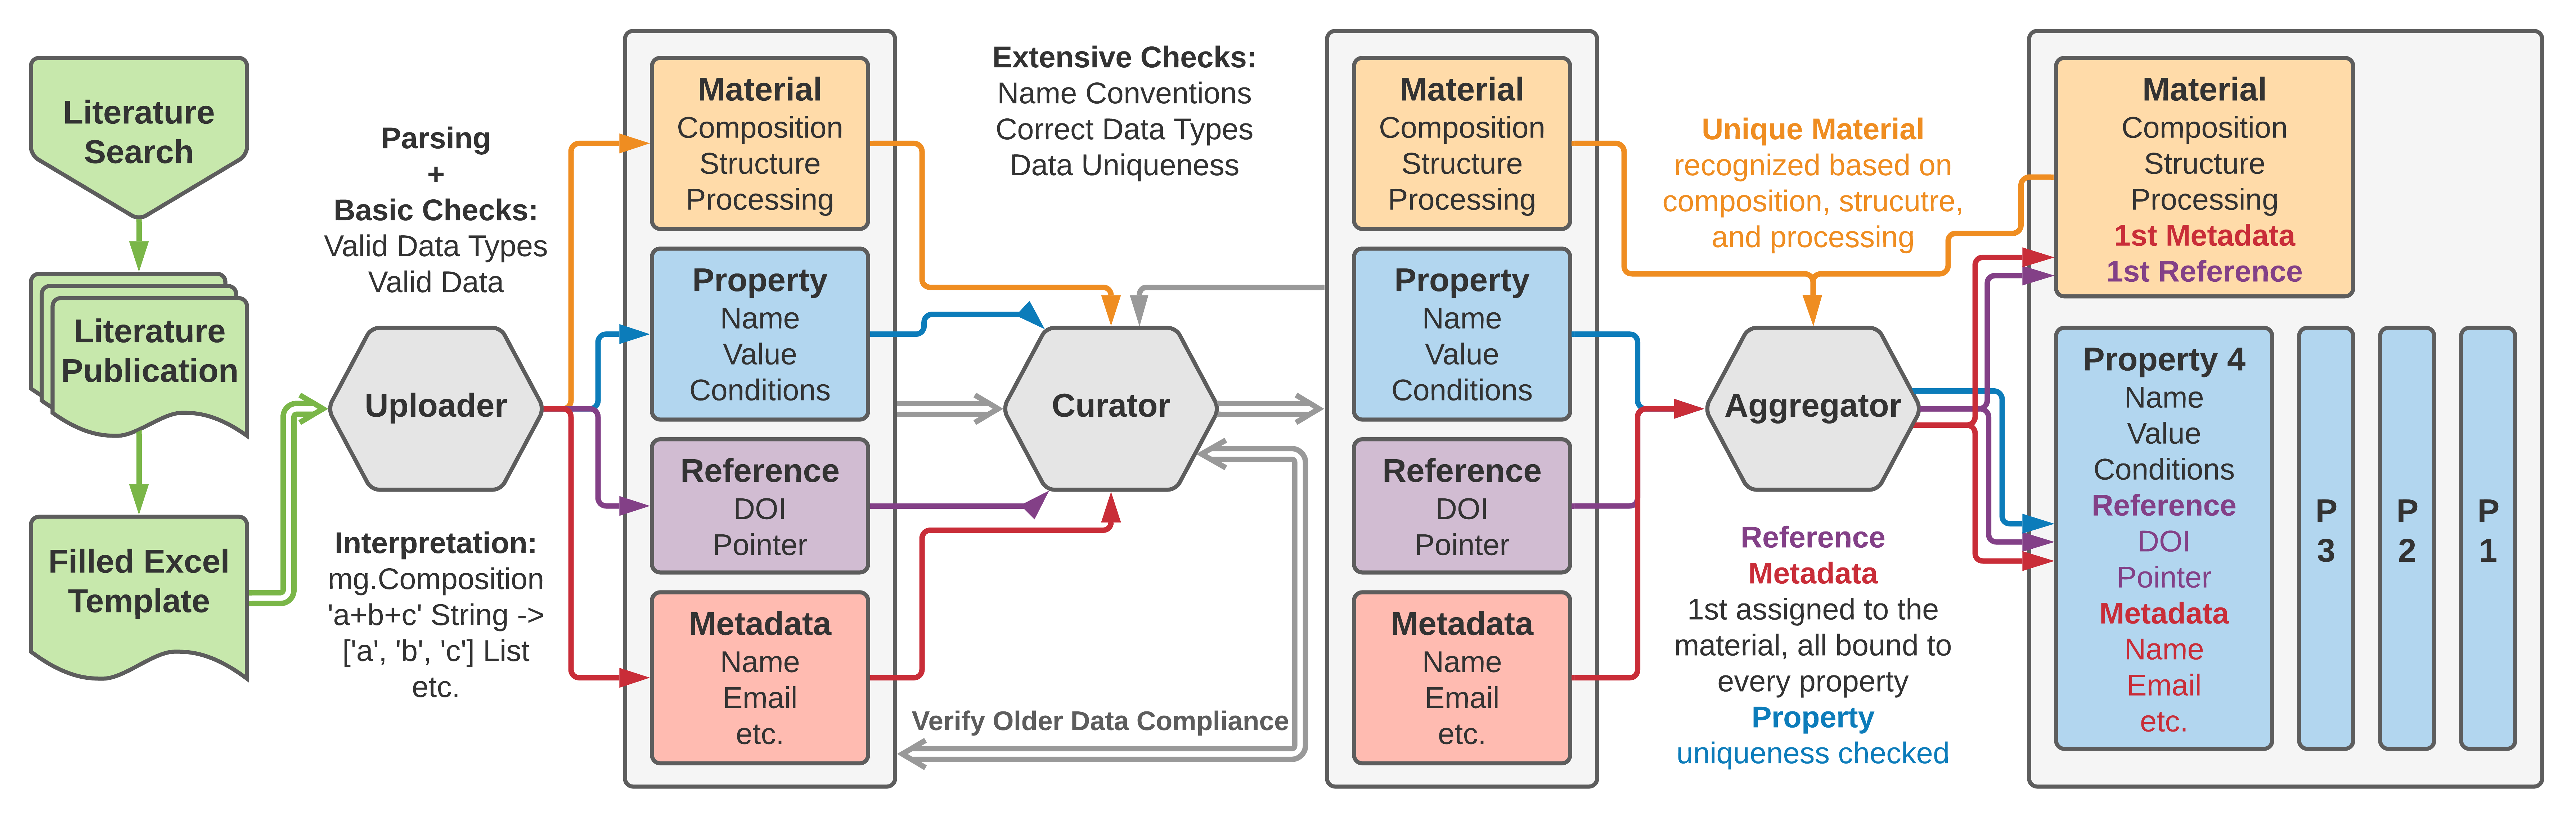
\includegraphics[width=0.95\textwidth]{ultera/ULTERA Data Detail.png}
    \caption{Schematic of the forward pipeline applied to data ingested into the system. For conciseness, intermediate steps of curation process and associated intermediate datasets are not depicted. Critically, a number of data points can converge at each step, so backward trace would be highly branched.}
    \label{ultera:fig:datapipeline}
\end{figure}


\begin{figure}[H]
    \centering
    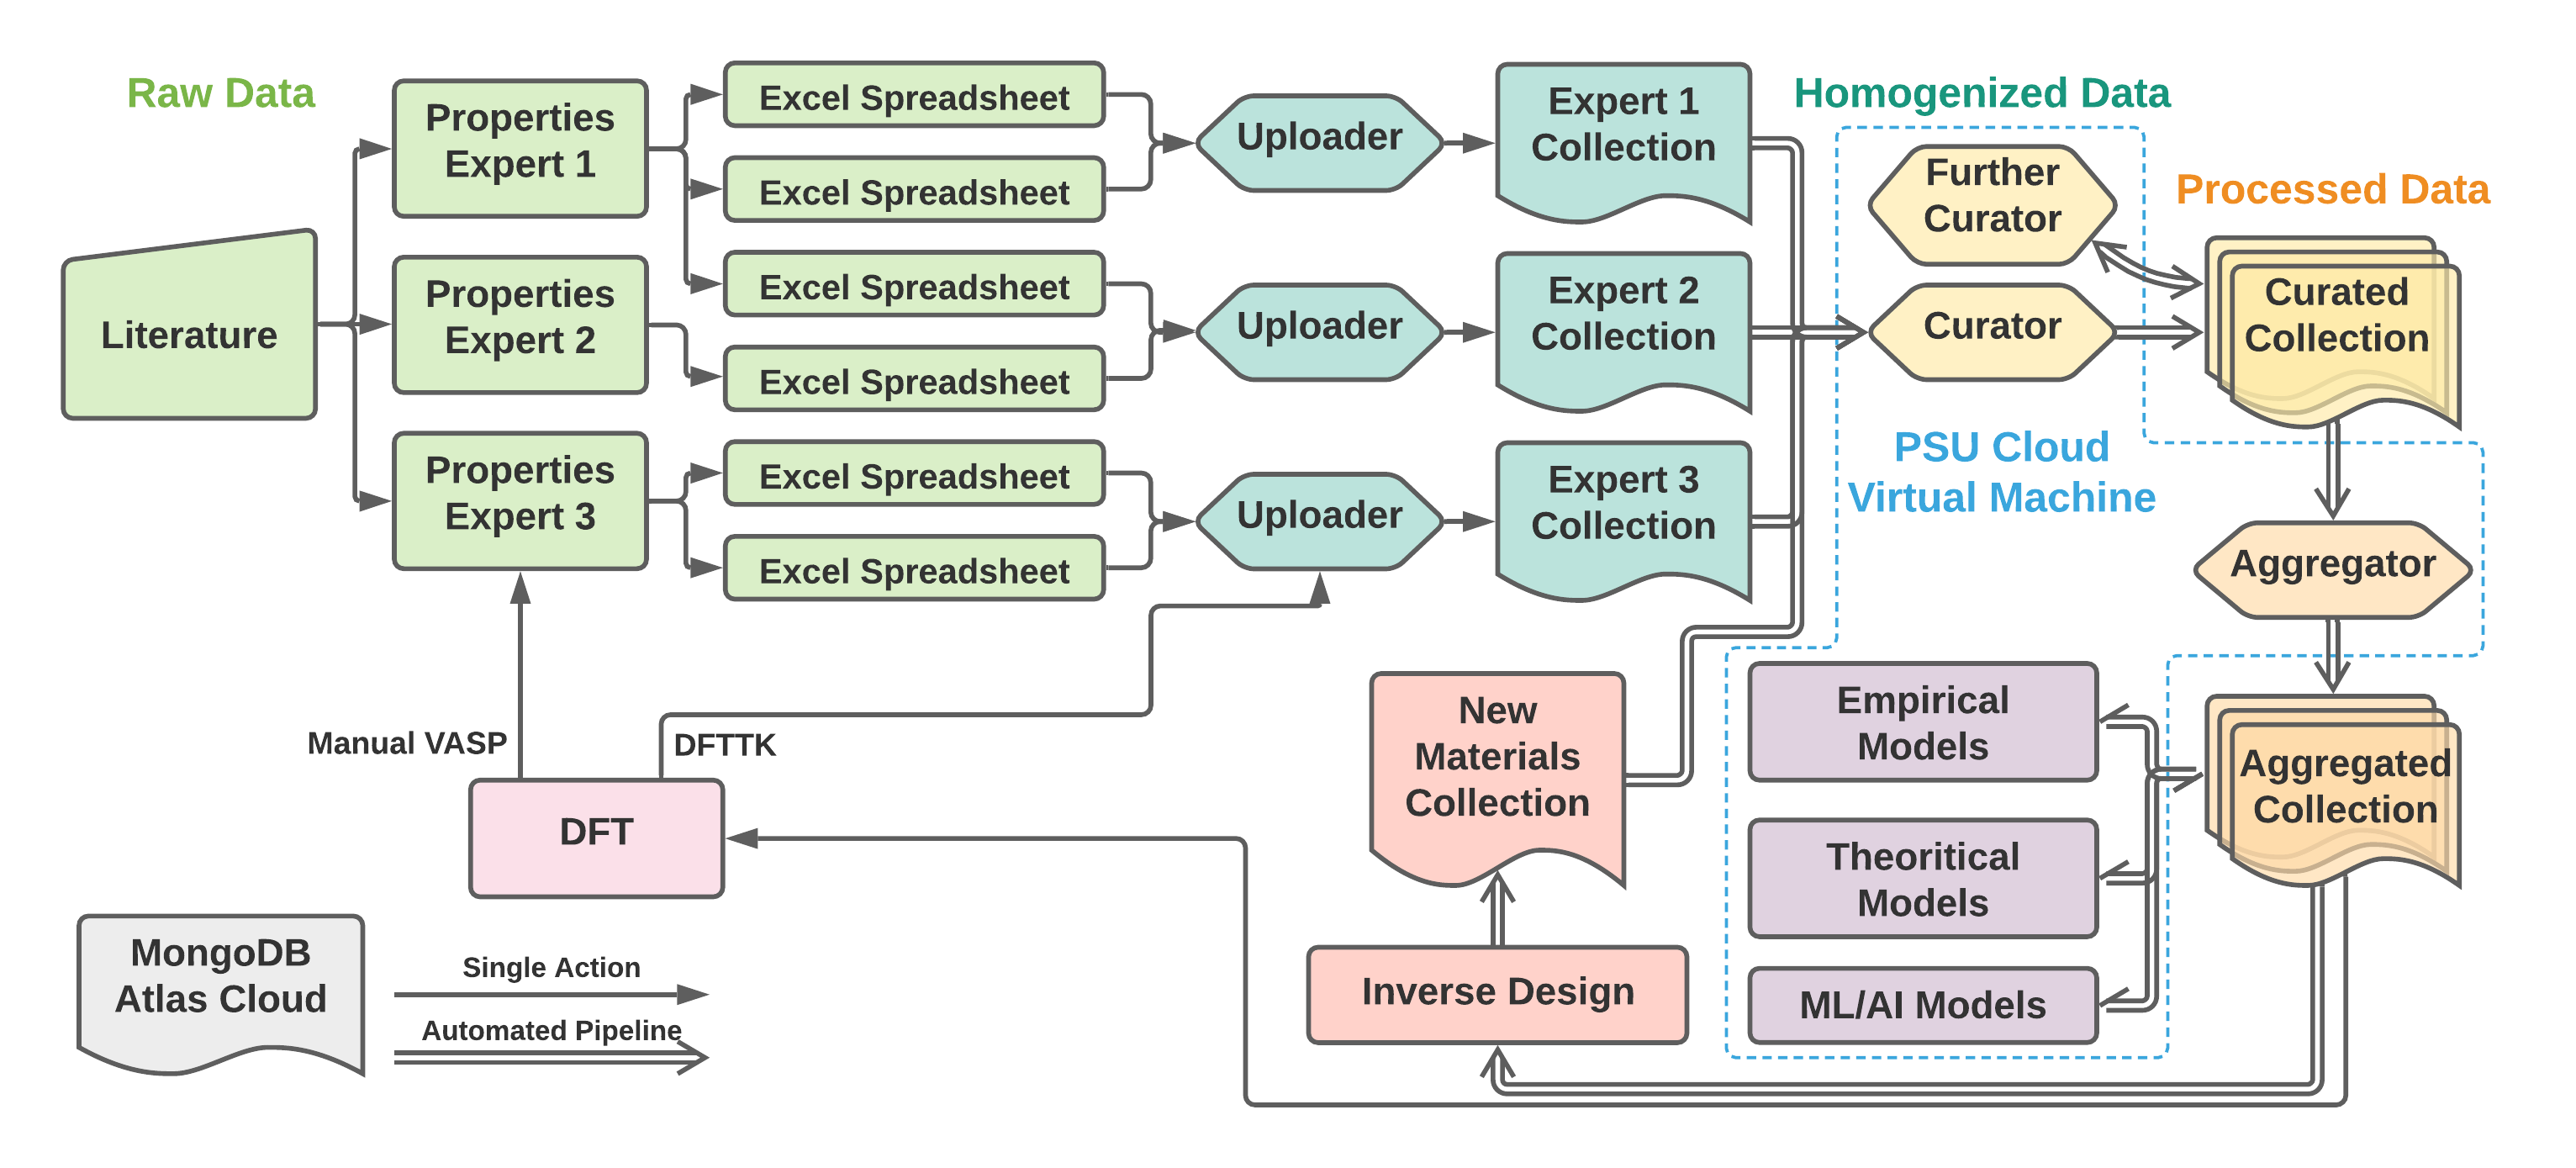
\includegraphics[width=0.95\textwidth]{ultera/ULTERA_Data_Cycle_v2.png}
    \caption{Schematic of the computational (non-experimental) data flow from perspective closer to the underlying pipelines, with double lines marking fully automated steps happening on the cloud. For conciseness, intermediate steps, like reorientation of data around unique compositional or structural datasets for efficient model deployment are not depicted.}
    \label{ultera:fig:datacycles}
\end{figure}




\section{Community Contributions} \label{ultera:sec:contributions}

\todo



\begin{figure}[H]
    \centering
    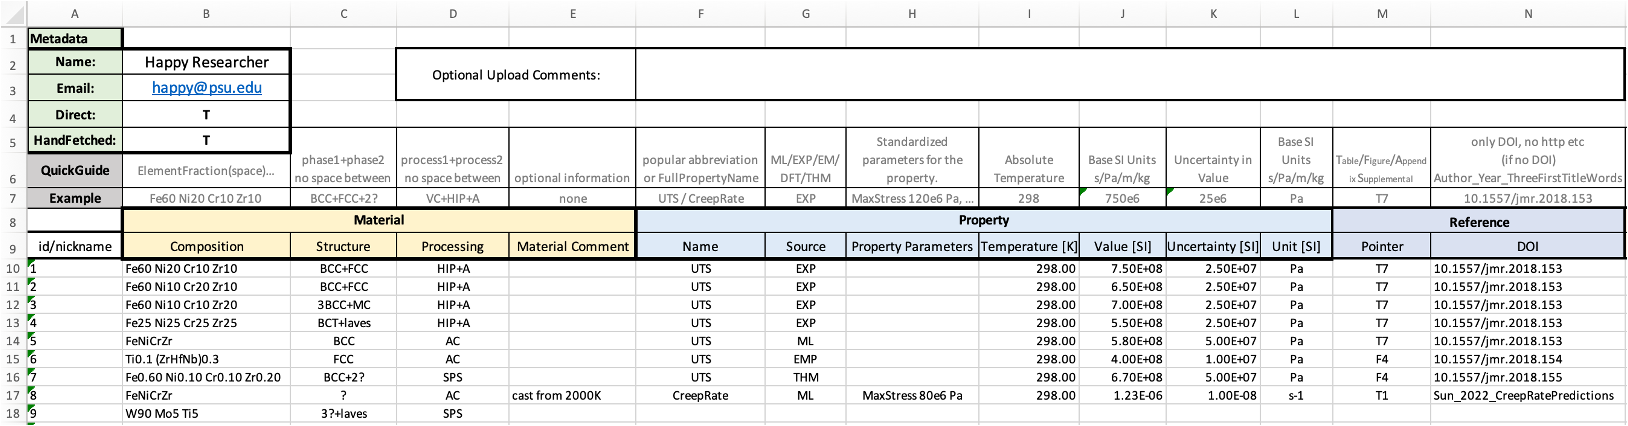
\includegraphics[width=0.95\textwidth]{ultera/ULTERA_Contribute.png}
    \caption{Header and example data rows of a formatted Excel spreadsheet template used to streamline and increase accessibility to the contribution system for non-technical members of the community. An automated system processes them on the cloud into git-tracked plain-text CSV records then passed to uploading system.}
    \label{ultera:fig:contributiontemplate}
\end{figure}




\section{Automatic Modeling} \label{ultera:sec:automodel}

\subsection{Multi-Structure Linear Combinations} \label{ultera:ssec:autolc}

\cite{Chong2021CorrelationAlloys}

\begin{figure}[H]
    \centering
    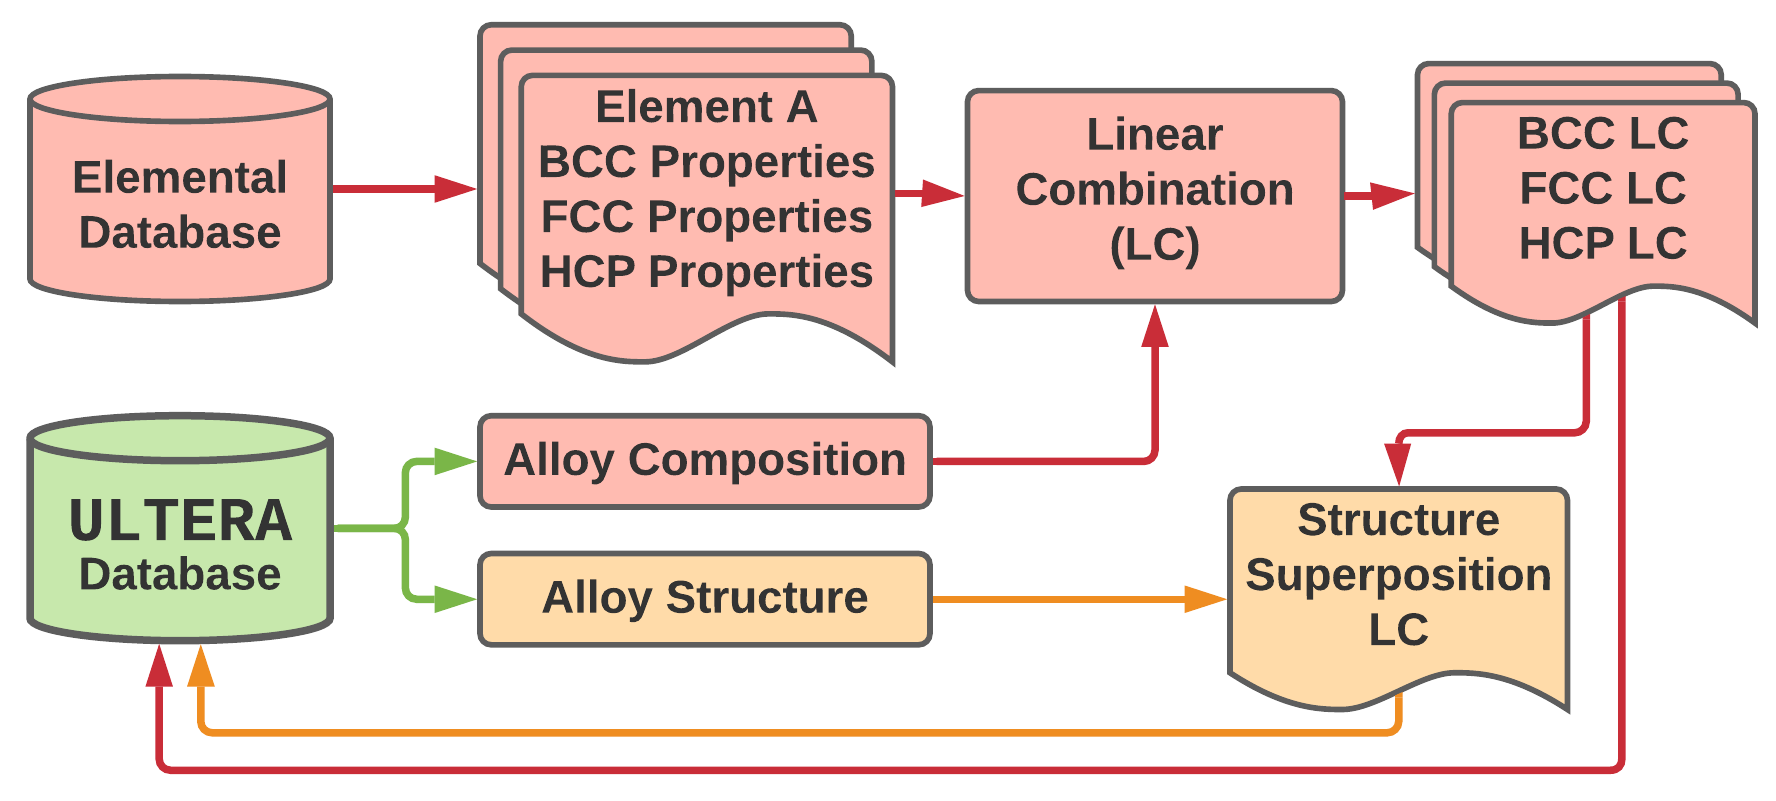
\includegraphics[width=0.6\textwidth]{ultera/ULTERA_ElementalDatabase_LC_V1.png}
    \caption{Simplified schematic of automatic linear combination modeling of properties. For every chemical composition, a linear combination of elemental properties is calculated for BCC, FCC, and HCP structures, based on best-matched elemental polymorph data coming from experiments and DFT-based pure element calculations. If applicable structure set (e.g., FCC+FCC+HCP) has been reported for a given input datapoint, an average of the respective linear combinations is reported as structure-informed LC.}
    \label{ultera:fig:autolc}
\end{figure}




\subsection{Community Model Deployment} \label{ultera:ssec:communitymodels}

\todo




\subsection{Automated CALPHAD Modeling} \label{ultera:ssec:autocalphad}

\todo






\subsection{MPDD Atomic Configuration Data Fetching} \label{ultera:ssec:mpdd}

\todo

\begin{figure}[H]
    \centering
    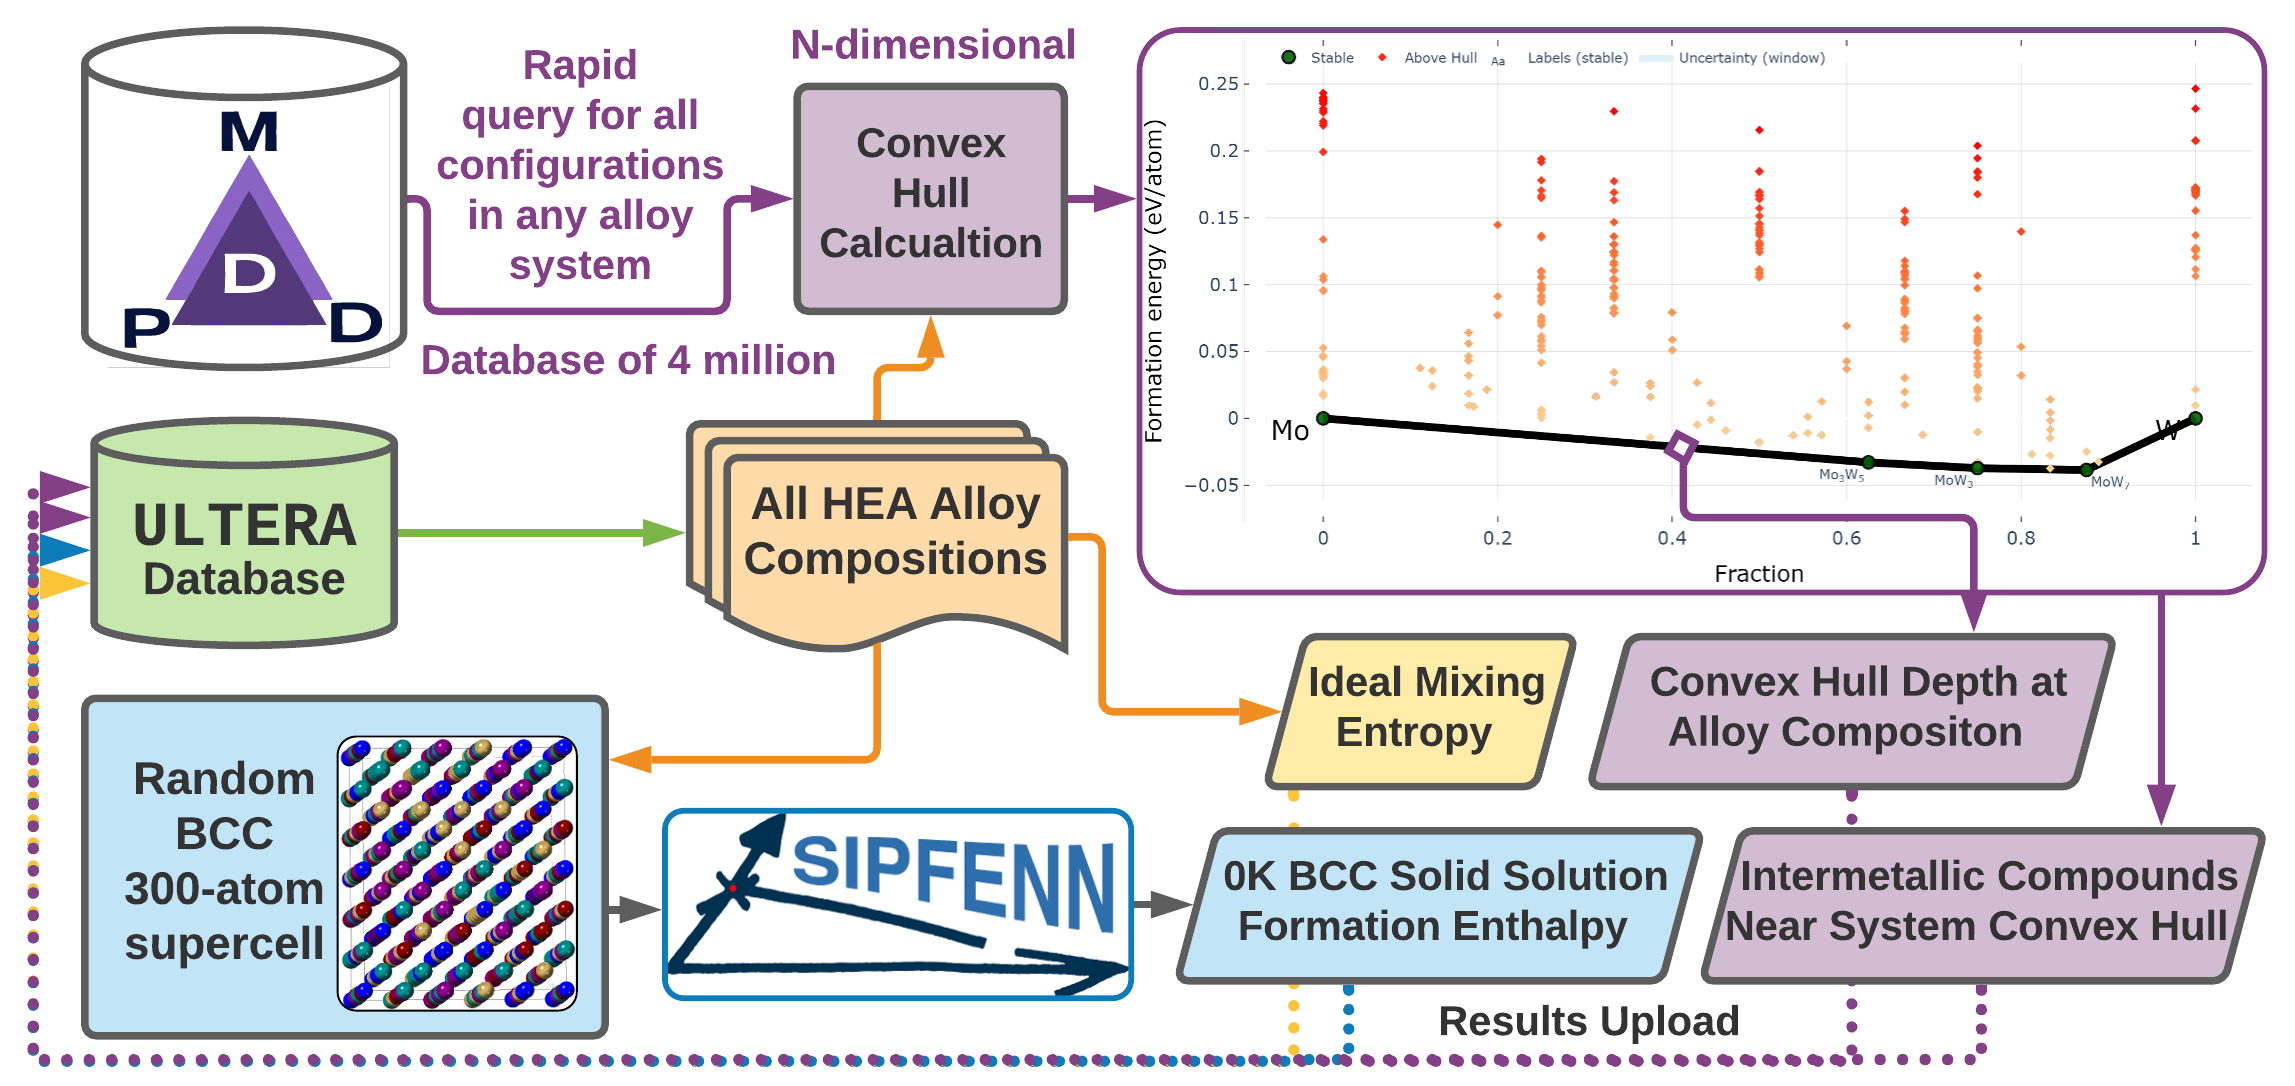
\includegraphics[width=0.6\textwidth]{ultera/ULTERA_BasicThermodynamics_V1.png}
    \caption{Conceptual schematic of how MPDD is directly utilized within ULTERA, going beyond interaction through CALPHAD models, to include basic thermodynamic information. For each composition, a convex hull of compounds present in corresponding chemical system is calculated based on MPDD data and can be used (a) to immediately identify candidates for experimentally observed compounds based on 0K low-energy configurations or (b) convex hull depth can be used as an input to ML model indicating strength of interatomic interactions.}
    \label{ultera:fig:mpdd}
\end{figure}








\printbibliography[heading=subbibintoc]